% \u5730\u652f\u5211\u5bb3\u7834\u5173\u7cfb\u603b\u89c8\u56fe
% \u7528\u9014\uff1a\u5c06\u5211\u3001\u5bb3\u3001\u7834\u4e09\u79cd\u7ec6\u5173\u7cfb\u653e\u5728\u4e00\u5f20\u56fe\u4e2d\uff0c\u4fbf\u4e8e\u590d\u4e60\u5bf9\u6bd4
\documentclass[tikz,border=10pt]{standalone}
\usepackage{ctex}
\usepackage{xcolor}
\pagecolor{white}
\usetikzlibrary{arrows.meta, positioning, calc, decorations.pathmorphing, backgrounds}

\begin{document}
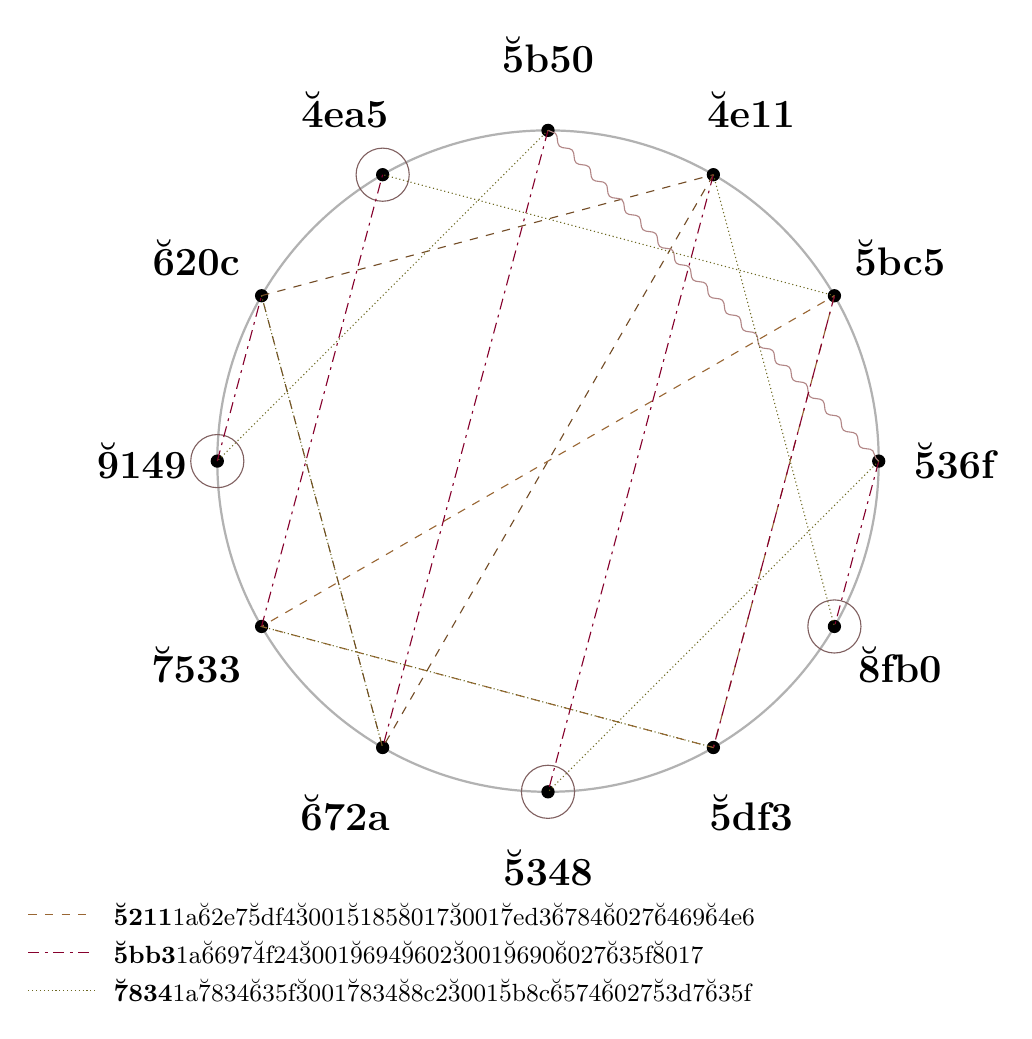
\begin{tikzpicture}[scale=1.2]
  \coordinate (zi)  at ( 90:3.5);
  \coordinate (chou) at ( 60:3.5);
  \coordinate (yin)  at ( 30:3.5);
  \coordinate (mao)  at (  0:3.5);
  \coordinate (chen) at (330:3.5);
  \coordinate (si)   at (300:3.5);
  \coordinate (wu)   at (270:3.5);
  \coordinate (wei)  at (240:3.5);
  \coordinate (shen) at (210:3.5);
  \coordinate (you)  at (180:3.5);
  \coordinate (xu)   at (150:3.5);
  \coordinate (hai)  at (120:3.5);

  \draw[thick, gray!60] (0,0) circle (3.5);

  \foreach \name/\angle/\text in {
    zi/90/\u5b50, chou/60/\u4e11, yin/30/\u5bc5, mao/0/\u536f,
    chen/330/\u8fb0, si/300/\u5df3, wu/270/\u5348, wei/240/\u672a,
    shen/210/\u7533, you/180/\u9149, xu/150/\u620c, hai/120/\u4ea5
  } {
    \fill[black] (\angle:3.5) circle (2pt);
    \node[font=\Large\bfseries] at (\angle:4.3) {\text};
  }

  % === \u5211\uff1a\u865a\u7ebf/\u6ce2\u6d6a\u7ebf/\u81ea\u73af ===
  % \u5bc5\u5df3\u7533\u4e09\u5211
  \draw[brown!80!black, thin, dashed] (yin) -- (si) -- (shen) -- cycle;
  % \u4e11\u672a\u620c\u4e09\u5211
  \draw[brown!60!black, thin, dashed] (chou) -- (wei) -- (xu) -- cycle;
  % \u5b50\u536f\u76f8\u5211
  \draw[pink!70!black, thin, decorate, decoration={snake, amplitude=0.4mm, segment length=3mm}] (zi) -- (mao);
  % \u81ea\u5211
  \foreach \angle in {330, 270, 180, 120} {
    \draw[pink!50!black, thin] (\angle:3.5) circle (8pt);
  }

  % === \u5bb3\uff1a\u70b9\u5212\u7ebf ===
  \draw[purple!70!black, thin, dash pattern=on 4pt off 2pt on 1pt off 2pt] (zi)   -- (wei);
  \draw[purple!70!black, thin, dash pattern=on 4pt off 2pt on 1pt off 2pt] (chou) -- (wu);
  \draw[purple!70!black, thin, dash pattern=on 4pt off 2pt on 1pt off 2pt] (yin)  -- (si);
  \draw[purple!70!black, thin, dash pattern=on 4pt off 2pt on 1pt off 2pt] (mao)  -- (chen);
  \draw[purple!70!black, thin, dash pattern=on 4pt off 2pt on 1pt off 2pt] (shen) -- (hai);
  \draw[purple!70!black, thin, dash pattern=on 4pt off 2pt on 1pt off 2pt] (you)  -- (xu);

  % === \u7834\uff1a\u77ed\u865a\u7ebf ===
  \draw[olive!70!black, thin, densely dotted] (zi)   -- (you);
  \draw[olive!70!black, thin, densely dotted] (chou) -- (chen);
  \draw[olive!70!black, thin, densely dotted] (yin)  -- (hai);
  \draw[olive!70!black, thin, densely dotted] (mao)  -- (wu);
  \draw[olive!70!black, thin, densely dotted] (shen) -- (si);
  \draw[olive!70!black, thin, densely dotted] (xu)   -- (wei);

  % \u56fe\u4f8b
  \draw[brown!80!black, thin, dashed] (-5.5,-4.8) -- (-4.8,-4.8);
  \node[font=\small, anchor=west] at (-4.7,-4.8) {\textbf{\u5211}\uff1a\u62e7\u5df4\u3001\u5185\u8017\u3001\u7ed3\u6784\u6027\u6469\u64e6};
  \draw[purple!70!black, thin, dash pattern=on 4pt off 2pt on 1pt off 2pt] (-5.5,-5.2) -- (-4.8,-5.2);
  \node[font=\small, anchor=west] at (-4.7,-5.2) {\textbf{\u5bb3}\uff1a\u6697\u4f24\u3001\u9694\u9602\u3001\u9690\u6027\u635f\u8017};
  \draw[olive!70!black, thin, densely dotted] (-5.5,-5.6) -- (-4.8,-5.6);
  \node[font=\small, anchor=west] at (-4.7,-5.6) {\textbf{\u7834}\uff1a\u7834\u635f\u3001\u7834\u88c2\u3001\u5b8c\u6574\u6027\u53d7\u635f};

  % \u767d\u8272\u80cc\u666f\uff0c\u9632\u6b62 GitHub dark mode \u4e0b\u900f\u660e SVG \u770b\u4e0d\u6e05
  \begin{scope}[on background layer]
    \fill[white] (current bounding box.south west) rectangle (current bounding box.north east);
  \end{scope}
\end{tikzpicture}
\end{document}
